\documentclass[tikz,border=5mm]{standalone}
\usepackage[T1]{fontenc}
\usepackage{lmodern}
\usepackage{amsmath,amssymb}
\usepackage{xcolor}
\usepackage{tikz}
\usetikzlibrary{arrows.meta,positioning,calc,fit,backgrounds,decorations.pathreplacing,shapes.geometric}
\tikzset{
  sknode/.style = {rectangle, draw, rounded corners=3pt, minimum width=2.0cm,
                   minimum height=0.85cm, align=center, inner sep=3pt,
                   font=\sffamily\fontsize{8.5}{10}\selectfont},
  mergelabel/.style = {rectangle, draw=black!40, fill=white, rounded corners=2pt,
                       minimum width=1.6cm, minimum height=0.55cm, align=center,
                       inner sep=2pt, font=\sffamily\fontsize{7.5}{9}\selectfont},
  regimelabel/.style = {font=\sffamily\bfseries\fontsize{9}{10.5}\selectfont},
}
\definecolor{regCalm}{HTML}{4C78A8}
\definecolor{regSpike}{HTML}{F58518}
\definecolor{leafgreen}{HTML}{54A24B}
\begin{document}
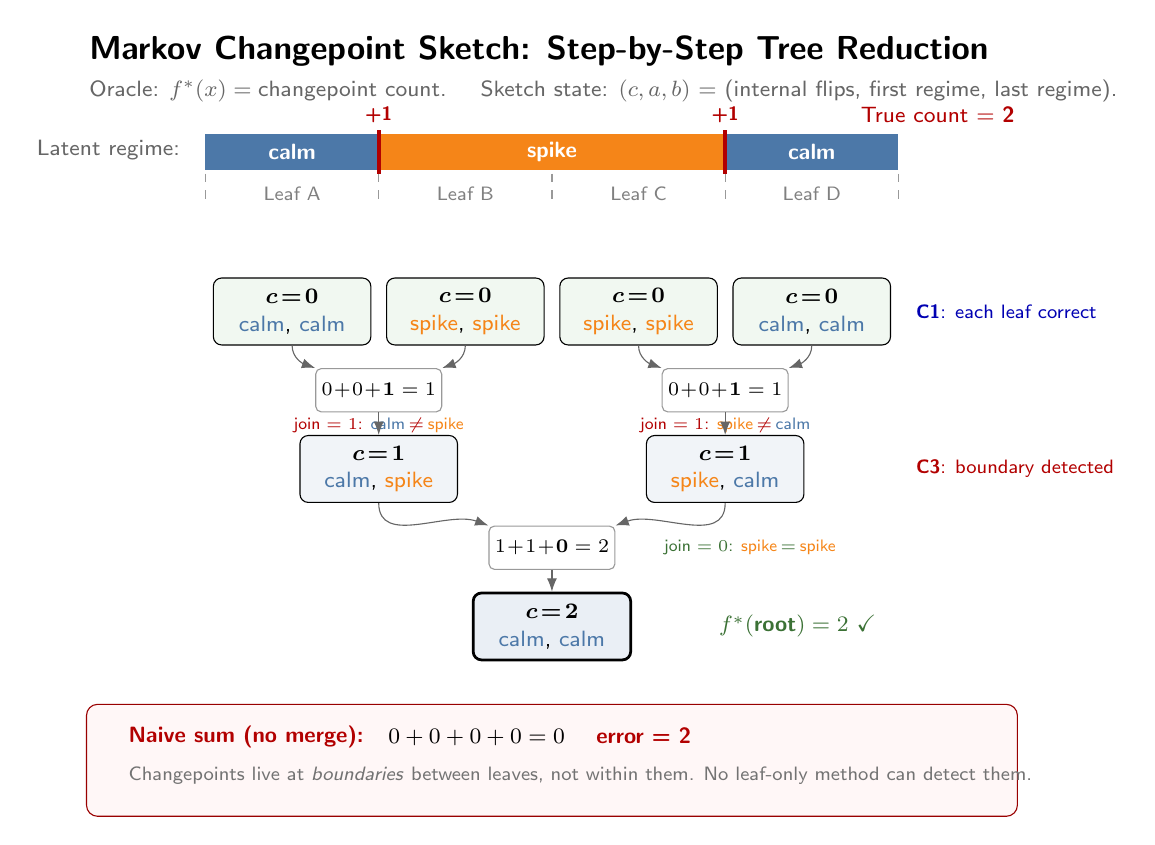
\begin{tikzpicture}[x=1cm,y=1cm,font=\sffamily,>=Latex]

  % Title
  \node[anchor=west, font=\sffamily\bfseries\fontsize{12}{14}\selectfont] at (0, 8.3)
    {Markov Changepoint Sketch: Step-by-Step Tree Reduction};

  % Subtitle
  \node[anchor=west, text=black!60, font=\sffamily\fontsize{8.5}{10}\selectfont] at (0, 7.8)
    {Oracle: $f^\ast(x) = \text{changepoint count}$. \quad
     Sketch state: $(c, a, b)$ = (internal flips, first regime, last regime).};

  % === Regime strip ===
  \node[anchor=east, font=\sffamily\fontsize{8.5}{10}\selectfont, text=black!60] at (1.4, 7.05)
    {Latent regime:};

  \fill[regCalm] (1.6, 6.8) rectangle ++(2.2, 0.45);
  \node[font=\sffamily\bfseries\fontsize{8.5}{10}\selectfont, text=white] at (2.7, 7.025) {calm};

  \fill[regSpike] (3.8, 6.8) rectangle ++(4.4, 0.45);
  \node[font=\sffamily\bfseries\fontsize{8.5}{10}\selectfont, text=white] at (6.0, 7.025) {spike};

  \fill[regCalm] (8.2, 6.8) rectangle ++(2.2, 0.45);
  \node[font=\sffamily\bfseries\fontsize{8.5}{10}\selectfont, text=white] at (9.3, 7.025) {calm};

  % Leaf boundaries
  \foreach \x/\lab in {1.6/A, 3.8/B, 6.0/C, 8.2/D} {
    \draw[black!40, dashed] (\x, 6.75) -- (\x, 6.4);
  }
  \draw[black!40, dashed] (10.4, 6.75) -- (10.4, 6.4);

  % Leaf labels
  \foreach \x/\lab in {2.7/A, 4.9/B, 7.1/C, 9.3/D} {
    \node[font=\sffamily\fontsize{7.5}{9}\selectfont, text=black!50] at (\x, 6.5) {Leaf \lab};
  }

  % Changepoint markers
  \draw[red!70!black, line width=1.5pt] (3.8, 6.75) -- (3.8, 7.3);
  \node[font=\sffamily\fontsize{7}{8.5}\selectfont, text=red!70!black] at (3.8, 7.5) {\textbf{+1}};
  \draw[red!70!black, line width=1.5pt] (8.2, 6.75) -- (8.2, 7.3);
  \node[font=\sffamily\fontsize{7}{8.5}\selectfont, text=red!70!black] at (8.2, 7.5) {\textbf{+1}};

  % True count annotation
  \node[anchor=east, font=\sffamily\fontsize{8}{9.5}\selectfont, text=red!70!black] at (12.0, 7.5)
    {True count = \textbf{2}};

  % === TREE ===

  % Level 0: Leaves
  \node[sknode, fill=leafgreen!8] (lA) at (2.7, 5.0)
    {$\boldsymbol{c\!=\!0}$\\ \textcolor{regCalm}{calm}, \textcolor{regCalm}{calm}};
  \node[sknode, fill=leafgreen!8] (lB) at (4.9, 5.0)
    {$\boldsymbol{c\!=\!0}$\\ \textcolor{regSpike}{spike}, \textcolor{regSpike}{spike}};
  \node[sknode, fill=leafgreen!8] (lC) at (7.1, 5.0)
    {$\boldsymbol{c\!=\!0}$\\ \textcolor{regSpike}{spike}, \textcolor{regSpike}{spike}};
  \node[sknode, fill=leafgreen!8] (lD) at (9.3, 5.0)
    {$\boldsymbol{c\!=\!0}$\\ \textcolor{regCalm}{calm}, \textcolor{regCalm}{calm}};

  % C1 annotation
  \node[font=\sffamily\fontsize{7}{8.5}\selectfont, text=blue!70!black, anchor=west] at (10.5, 5.0)
    {\textbf{C1}: each leaf correct};

  % Level 1: First merges
  \node[sknode, fill=regCalm!8] (mAB) at (3.8, 3.0)
    {$\boldsymbol{c\!=\!1}$\\ \textcolor{regCalm}{calm}, \textcolor{regSpike}{spike}};
  \node[sknode, fill=regCalm!8] (mCD) at (8.2, 3.0)
    {$\boldsymbol{c\!=\!1}$\\ \textcolor{regSpike}{spike}, \textcolor{regCalm}{calm}};

  % Merge computation labels
  \node[mergelabel] (cAB) at (3.8, 4.0)
    {$0\!+\!0\!+\!\mathbf{1}=1$};
  \node[mergelabel] (cCD) at (8.2, 4.0)
    {$0\!+\!0\!+\!\mathbf{1}=1$};

  % Join annotations (placed below each merge box to avoid overlap)
  \node[font=\sffamily\fontsize{6.5}{8}\selectfont, text=red!70!black] at (3.8, 3.55)
    {join${}=1$: \textcolor{regCalm}{calm}$\,{\neq}\,$\textcolor{regSpike}{spike}};
  \node[font=\sffamily\fontsize{6.5}{8}\selectfont, text=red!70!black] at (8.2, 3.55)
    {join${}=1$: \textcolor{regSpike}{spike}$\,{\neq}\,$\textcolor{regCalm}{calm}};

  % C3 annotation
  \node[font=\sffamily\fontsize{7}{8.5}\selectfont, text=red!70!black, anchor=west] at (10.5, 3.0)
    {\textbf{C3}: boundary detected};

  % Edges: leaves to merge labels
  \draw[->, black!60] (lA.south) to[out=-90,in=160] (cAB.north west);
  \draw[->, black!60] (lB.south) to[out=-90,in=20] (cAB.north east);
  \draw[->, black!60] (lC.south) to[out=-90,in=160] (cCD.north west);
  \draw[->, black!60] (lD.south) to[out=-90,in=20] (cCD.north east);

  % Edges: merge labels to merge nodes
  \draw[->, black!60] (cAB.south) -- (mAB.north);
  \draw[->, black!60] (cCD.south) -- (mCD.north);

  % Level 2: Root
  \node[sknode, fill=regCalm!12, line width=1pt] (root) at (6.0, 1.0)
    {$\boldsymbol{c\!=\!2}$\\ \textcolor{regCalm}{calm}, \textcolor{regCalm}{calm}};
  \node[mergelabel] (cRoot) at (6.0, 2.0)
    {$1\!+\!1\!+\!\mathbf{0}=2$};

  % Join annotation for root
  \node[font=\sffamily\fontsize{6.5}{8}\selectfont, text=leafgreen!70!black, anchor=west] at (7.3, 2.0)
    {join${}=0$: \textcolor{regSpike}{spike}$\,{=}\,$\textcolor{regSpike}{spike}};

  % Edges: merge to root
  \draw[->, black!60] (mAB.south) to[out=-90,in=160] (cRoot.north west);
  \draw[->, black!60] (mCD.south) to[out=-90,in=20] (cRoot.north east);
  \draw[->, black!60] (cRoot.south) -- (root.north);

  % Result annotation
  \node[font=\sffamily\bfseries\fontsize{8.5}{10}\selectfont, text=leafgreen!70!black, anchor=west] at (8.0, 1.0)
    {$f^\ast(\text{root}) = 2$ \checkmark};

  % === NAIVE SUM COMPARISON ===
  \begin{scope}[on background layer]
    \node[draw=red!60!black, fill=red!3, rounded corners=4pt, inner sep=6pt,
          fit={(0.3,-0.2) (11.7,-1.2)}] (naivebox) {};
  \end{scope}
  \node[anchor=west, font=\sffamily\bfseries\fontsize{8.5}{10}\selectfont, text=red!70!black] at (0.5, -0.4)
    {Naive sum (no merge):};
  \node[anchor=west, font=\sffamily\fontsize{8.5}{10}\selectfont] at (3.8, -0.4)
    {$0 + 0 + 0 + 0 = 0$ \quad\textcolor{red!70!black}{\textbf{error = 2}}};
  \node[anchor=west, font=\sffamily\fontsize{7.5}{9}\selectfont, text=black!55] at (0.5, -0.9)
    {Changepoints live at \emph{boundaries} between leaves, not within them.
     No leaf-only method can detect them.};

\end{tikzpicture}
\end{document}
